% !TeX spellcheck = en_US
\addsection{Components}{\skills/luck.png}

This is a visual guide of what is what, and shows components from every expansion together. Please refer to the official component lists for the exact numbers and pictures of all individual components.

\vspace*{-1em}
\begin{figure}[H]
  \centering
  \begin{subfigure}[b]{0.4\linewidth}
    \includegraphics[width=\linewidth]{\images/combat_board_2.png}
    \caption{\textbf{Combat Board}}
  \end{subfigure}
  ~
  \begin{subfigure}[b]{0.5\linewidth}
    \includegraphics[width=\linewidth]{\images/battlefield-alone.png}
    \caption{\textbf{Battlefield Board} (Battlefield Expansion)}
  \end{subfigure}
\end{figure}
\vspace*{-1.5em}
\begin{figure}[H]
  \centering
  \begin{subfigure}[b]{0.25\linewidth}
    \includegraphics[width=\linewidth]{\images/hero.png}
    \caption{\textbf{Hero Card}}
  \end{subfigure}
  ~
  \begin{subfigure}[b]{0.25\linewidth}
    \includegraphics[width=\linewidth]{\images/town.png}
    \caption{\textbf{Town Board}}
  \end{subfigure}
  ~
  \begin{subfigure}[b]{0.25\linewidth}
    \centering
    \includegraphics[width=\linewidth]{\images/map-tile-back.png}
    \caption{\textbf{Map tile}}
  \end{subfigure}
  ~
  \begin{subfigure}[b]{0.15\linewidth}
    \centering
    \includegraphics[width=\linewidth]{\images/grail.png}
    \caption{\textbf{Grail Token}}
  \end{subfigure}
\end{figure}
\vspace*{-1.7em}
\begin{figure}[H]
  \centering
  \begin{subfigure}[b]{0.16\linewidth}
    \centering
    \includegraphics[width=0.6\linewidth]{\images/initiative-bf.png}
    \caption{\textbf{Initiative Token} (Battlefield Expansion)}
  \end{subfigure}
  \begin{subfigure}[b]{0.18\linewidth}
    \centering
    \includegraphics[width=\linewidth]{\images/gold-tokens.png}
    \caption{\textbf{Gold Tokens} \phantom{Population} \phantom{Population} \phantom{Population}}
  \end{subfigure}
  \begin{subfigure}[b]{0.12\linewidth}
    \centering
    \includegraphics[width=0.6\linewidth]{\images/building-materials-token.png}
    \caption{\textbf{Building Materials Token} \phantom{Population}}
  \end{subfigure}
  \begin{subfigure}[b]{0.12\linewidth}
    \centering
    \includegraphics[width=0.6\linewidth]{\images/valuables-token.png}
    \caption{\textbf{Valuables Token} \phantom{Population} \phantom{Population}}
  \end{subfigure}
  \begin{subfigure}[b]{0.12\linewidth}
    \centering
    \includegraphics[width=5em]{\images/build.png}
    \caption{\textbf{Build Token} \phantom{Population} \phantom{Population}}
  \end{subfigure}
  \begin{subfigure}[b]{0.13\linewidth}
    \centering
    \includegraphics[width=5em]{\images/population.png}
    \caption{\textbf{Population Token} \phantom{Population} \phantom{Population}}
  \end{subfigure}
  \begin{subfigure}[b]{0.12\linewidth}
    \centering
    \includegraphics[width=5em]{\images/spells.png}
    \caption{\textbf{Spell Book Token} \phantom{Population}}
  \end{subfigure}
\end{figure}
\vspace*{-4em}
\begin{figure}[H]
  \centering
  \begin{subfigure}[b]{0.2\linewidth}
    \begin{tikzpicture}
      \node at (0, 0) {\includegraphics[width=0.6\linewidth]{\images/morale-negative.png}};
      \node at (1, 0) {\includegraphics[width=0.6\linewidth]{\images/morale-positive.png}};
    \end{tikzpicture}
    \caption{\textbf{Morale Token}}
  \end{subfigure}
  \begin{subfigure}[b]{0.1\linewidth}
    \centering
    \includegraphics[width=3em]{\images/damage-token.png}
    \caption{\textbf{Damage Token}}
  \end{subfigure}
  \begin{subfigure}[b]{0.17\linewidth}
    \centering
    \includegraphics[width=4.5em]{\images/paralysis-defense.png}
    \caption{\textbf{Paralysis/ Defense Token}}
  \end{subfigure}
  \begin{subfigure}[b]{0.15\linewidth}
    \centering
    \includesvg[width=\linewidth]{\images/movement_tokens.svg}
    \caption{\textbf{Movement Tokens}}
  \end{subfigure}
  \begin{subfigure}[b]{0.15\linewidth}
    \centering
    \includegraphics[width=0.8\linewidth]{\images/blue-cubes.png}
    \includegraphics[width=0.8\linewidth]{\images/purple-cubes.png}
    \caption{\textbf{Faction cubes}}
  \end{subfigure}
  \begin{subfigure}[b]{0.15\linewidth}
    \centering
    \includegraphics[width=\linewidth]{\images/black-cubes.png}
    \caption{\textbf{Black cubes}}
  \end{subfigure}
\end{figure}
\vspace*{-2em}
\begin{figure}[H]
  \centering
  \begin{subfigure}[b]{0.25\linewidth}
    \begin{tikzpicture}
      \node at (0, 0) {\includegraphics[width=0.6\linewidth]{\cards/morale-positive-back.png}};
      \node at (1.5, 0.1) {\includegraphics[width=0.6\linewidth]{\cards/morale-positive.png}};
    \end{tikzpicture}
    \caption{\textbf{Positive Morale Card} (Battlefield Expansion)}
  \end{subfigure}
  \begin{subfigure}[b]{0.25\linewidth}
    \begin{tikzpicture}
      \node at (0, 0) {\includegraphics[width=0.6\linewidth]{\cards/morale-negative-back.png}};
      \node at (1.5, 0.1) {\includegraphics[width=0.6\linewidth]{\cards/morale-negative.png}};
    \end{tikzpicture}
    \caption{\textbf{Negative Morale Card} (Battlefield Expansion)}
  \end{subfigure}
  \begin{subfigure}[b]{0.4\linewidth}
    \centering
    \includegraphics[width=\linewidth]{\images/hero-minis.png}
    \caption{\textbf{Hero miniatures}}
  \end{subfigure}
\end{figure}
\vspace*{-2em}

\clearpage

\vspace*{-4em}
\begin{figure}[H]
  \centering
  \begin{subfigure}[t]{0.23\linewidth}
    \centering
    \begin{tikzpicture}
      \node at (0, 0) {\includegraphics[width=0.8\linewidth]{\cards/event-back.png}};
      \node at (1, 1) {\includegraphics[width=0.8\linewidth]{\cards/event.png}};
    \end{tikzpicture}
    \caption{\textbf{Event Card}\\(Fortress Expansion)}
  \end{subfigure}
  ~
  \begin{subfigure}[t]{0.23\linewidth}
    \centering
    \begin{tikzpicture}
      \node at (0, 0) {\includegraphics[width=0.8\linewidth]{\cards/astrolog-back.png}};
      \node at (1, 1) {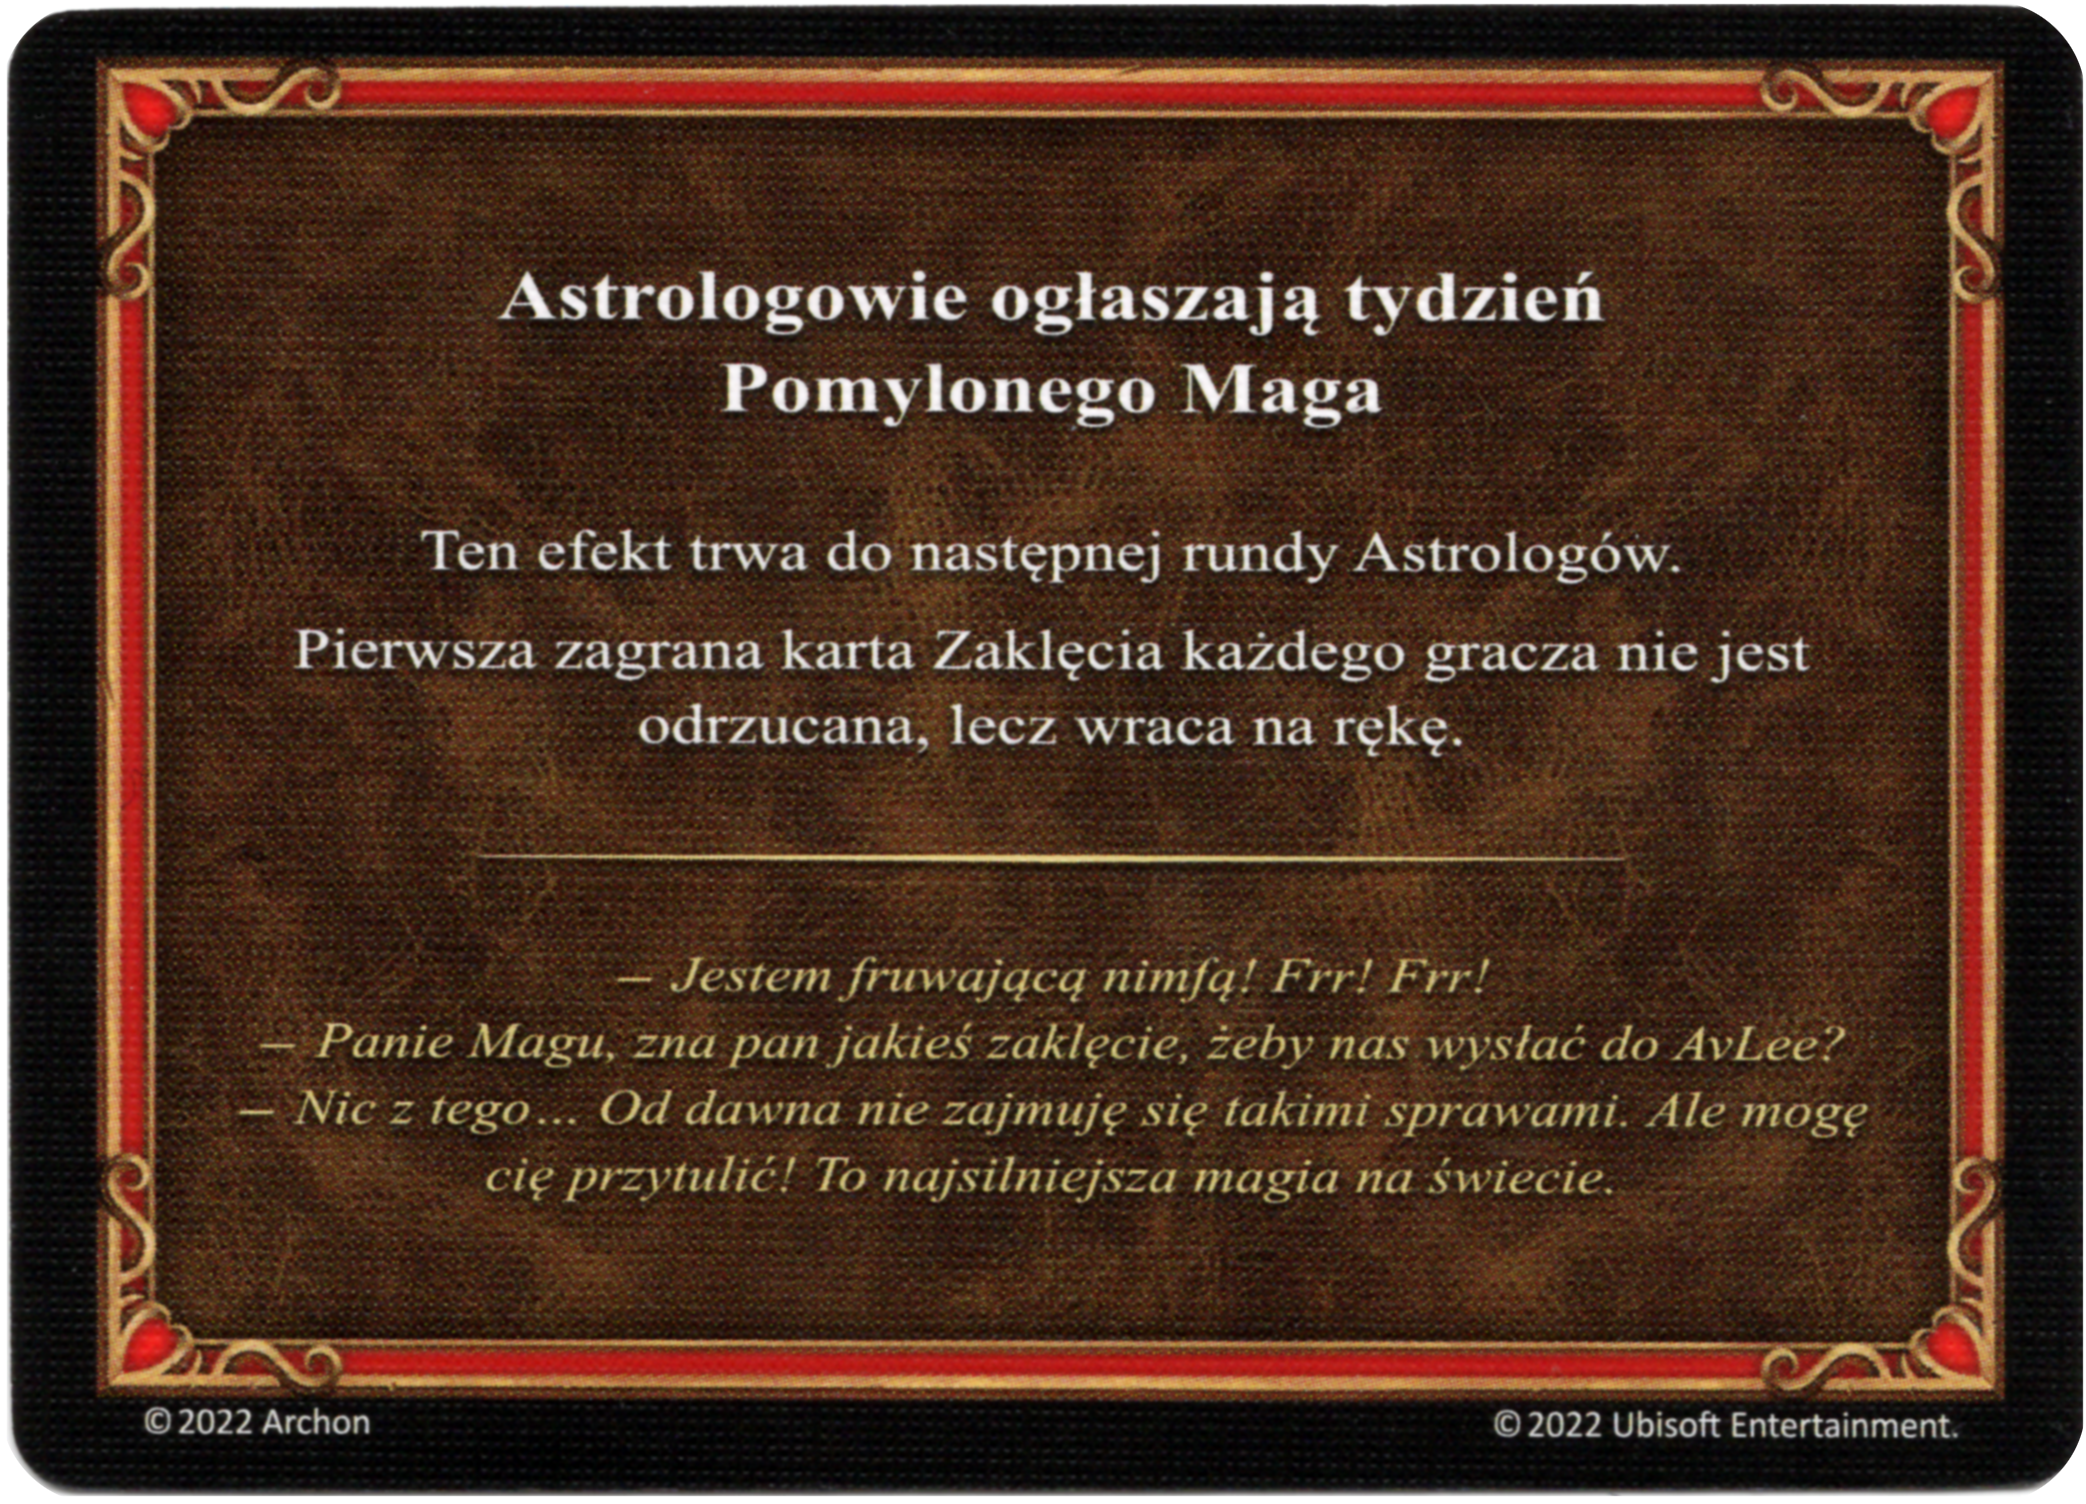
\includegraphics[width=0.8\linewidth]{\cards/astrolog.png}};
    \end{tikzpicture}
    \caption{\textbf{Astrologers Proclaim Card}}
  \end{subfigure}
  ~
  \begin{subfigure}[t]{0.23\linewidth}
    \centering
    \includegraphics[width=\linewidth]{\cards/aiback.png}
    \caption{\textbf{AI Card}}
  \end{subfigure}
  ~
  \begin{subfigure}[t]{0.23\linewidth}
    \centering
    \includegraphics[width=\linewidth]{\cards/adventure.png}
    \caption{\textbf{Adventure Card} (Battlefield Expansion)}
  \end{subfigure}
\end{figure}
\vspace*{-2em}
\begin{figure}[H]
  \centering
  \begin{subfigure}[t]{0.23\linewidth}
    \centering
    \begin{tikzpicture}
      \node at (0, 0) {\includegraphics[width=0.6\linewidth]{\cards/mmback.png}};
      \node at (1.5, 0.1) {\includegraphics[width=0.6\linewidth]{\cards/necromancy_card.png}};
    \end{tikzpicture}
    \caption{\textbf{Ability Card}}
  \end{subfigure}
  \begin{subfigure}[t]{0.23\linewidth}
    \centering
    \begin{tikzpicture}
      \node at (0, 0) {\includegraphics[width=0.6\linewidth]{\cards/mmback.png}};
      \node at (1.5, 0.1) {\includegraphics[width=0.6\linewidth]{\cards/artifact-front.png}};
    \end{tikzpicture}
    \caption{\textbf{Artifact Card}}
  \end{subfigure}
  \begin{subfigure}[t]{0.23\linewidth}
    \centering
    \begin{tikzpicture}
      \node at (0, 0) {\includegraphics[width=0.6\linewidth]{\cards/mmback.png}};
      \node at (1.5, 0.1) {\includegraphics[width=0.6\linewidth]{\cards/spell.png}};
    \end{tikzpicture}
    \caption{\textbf{Spell Card}}
  \end{subfigure}
\end{figure}
\vspace*{-2em}
\begin{figure}[H]
  \centering
  \begin{subfigure}[t]{0.23\linewidth}
    \centering
    \begin{tikzpicture}
      \node at (0, 0) {\includegraphics[width=0.6\linewidth]{\cards/mmback.png}};
      \node at (1.5, 0.1) {\includegraphics[width=0.6\linewidth]{\cards/war_machine.png}};
    \end{tikzpicture}
    \caption{\textbf{War Machine Card} (Rampart Expansion)}
  \end{subfigure}
  \begin{subfigure}[t]{0.23\linewidth}
    \centering
    \begin{tikzpicture}
      \node at (0, 0) {\includegraphics[width=0.6\linewidth]{\cards/mmback.png}};
      \node at (1.5, 0.1) {\includegraphics[width=0.6\linewidth]{\cards/specialty.png}};
    \end{tikzpicture}
    \caption{\textbf{Hero Specialty Card}}
  \end{subfigure}
  \begin{subfigure}[t]{0.23\linewidth}
    \centering
    \begin{tikzpicture}
      \node at (0, 0) {\includegraphics[width=0.6\linewidth]{\cards/mmback.png}};
      \node at (1.5, 0.1) {\includegraphics[width=0.6\linewidth]{\cards/statistic.png}};
    \end{tikzpicture}
    \caption{\textbf{Statistic Card}}
  \end{subfigure}
  \begin{subfigure}[t]{0.23\linewidth}
    \centering
    \begin{tikzpicture}
      \node at (0, 0) {\includegraphics[width=0.6\linewidth]{\cards/mmback.png}};
      \node at (1.5, 0.1) {\includegraphics[width=0.6\linewidth]{\cards/empowered_statistic.png}};
    \end{tikzpicture}
    \caption{\textbf{Empowered Statistic Card} (Inferno Expansion)}
  \end{subfigure}
\end{figure}
\vspace*{-3em}
\begin{figure}[H]
  \centering
  \begin{subfigure}[t]{0.23\linewidth}
    \centering
    \begin{tikzpicture}
      \node at (0, 0) {\includegraphics[width=0.6\linewidth]{\cards/neutral-back.png}};
      \node at (1.5, 0.1) {\includegraphics[width=0.6\linewidth]{\cards/neutral-front.png}};
    \end{tikzpicture}
    \caption{\textbf{Neutral Unit Card}}
  \end{subfigure}
  ~
  \begin{subfigure}[t]{0.23\linewidth}
    \centering
    \begin{tikzpicture}
      \node at (0, 0) {\includegraphics[width=0.6\linewidth]{\cards/unit-pack.png}};
      \node at (1.5, 0.1) {\includegraphics[width=0.6\linewidth]{\cards/unit-few.png}};
    \end{tikzpicture}
    \caption{\textbf{Faction Unit Card}}
  \end{subfigure}
  ~
  \begin{subfigure}[t]{0.23\linewidth}
    \centering
    \begin{tikzpicture}
      \node at (0, 0) {\includegraphics[width=0.6\linewidth]{\cards/arrow_tower_back.png}};
      \node at (1.5, 0.1) {\includegraphics[width=0.6\linewidth]{\cards/arrow_tower.png}};
    \end{tikzpicture}
    \caption{\textbf{Arrow Tower Card}}
  \end{subfigure}
  ~
  \begin{subfigure}[t]{0.23\linewidth}
    \centering
    \includegraphics[width=\linewidth]{\cards/gate.png}
    \caption{\textbf{Gate, Walls Cards}}
  \end{subfigure}
\end{figure}

\vspace*{-2em}
\columnratio{0.4}
\begin{paracol}{2}
\begin{figure}[H]
  \centering
  \begin{subfigure}[b]{0.3\linewidth}
    \centering
    \includegraphics[width=0.7\linewidth]{\images/attack_die.png}
    \caption{\textbf{Attack Dice}}
  \end{subfigure}
  \begin{subfigure}[b]{0.3\linewidth}
    \centering
    \includegraphics[width=\linewidth]{\images/treasure_die.png}
    \caption{\textbf{Treasure Dice}}
  \end{subfigure}
  \begin{subfigure}[b]{0.3\linewidth}
    \centering
    \includegraphics[width=0.8\linewidth]{\images/resource_die.png}
    \caption{\textbf{Resource Dice}}
  \end{subfigure}
\end{figure}
\vspace*{-1em}
\begin{figure}[H]
  \centering
  \begin{subfigure}[b]{\linewidth}
    \centering
    \includegraphics[width=0.8\linewidth]{\images/round-tracker.png}
    \caption{\textbf{Round Tracker}}
  \end{subfigure}
\end{figure}
\switchcolumn
\begin{figure}[H]
  \vspace*{1em}
  \centering
  \begin{subfigure}[b]{\linewidth}
    \centering
    \includegraphics[width=\linewidth]{\images/battlefield-obstacles.png}
    \caption{\textbf{Obstacles} (Battlefield Expansion)}
  \end{subfigure}
\end{figure}
\end{paracol}
